\noindent
The objective of this section is to validate the critical aspects of the Best Bike Paths (BBP) system using Alloy, a lightweight formal method based on relational logic. In particular, the modeling effort concentrates on the robustness of the report submission mechanism, a core feature for maintaining data reliability within the platform.
\subsection{Signatures}
The signatures defined below represent the vocabulary used to describe the BBP ecosystem. Here, we outline the primary atoms of the model, including User, Trip, and Path, while also defining the dynamic elements such as Obstacle and PathStatus that are essential for tracking the system's evolution.

\lstinputlisting[language=alloy]{RASD/Alloy/Signatures.txt}


\newpage
\subsection{Facts}
The facts represent the constraints that the system must respect and are always true in the model. For the BBP application, we defined numerous facts to enforce data consistency, such as the necessity for a PathReport to be strictly linked to a Trip performed by the author. Furthermore, they dictate the logic for the dynamic evolution of the system, determining how PathStatus and Obstacles are updated based on the aggregation of user reports.
\lstinputlisting[language=alloy]{RASD/Alloy/Facts.txt}

\subsection{Assertions}
The assertions are the safety properties that we want to verify in the model. These conditions must hold true to ensure the platform avoids invalid or illogical states. For the BBP scenario, we verified several critical aspects, such as the strict requirement that a User must have actually completed a Trip on a specific Path before submitting a report (AuthorWasThere), as well as the constraint that limits users to a single report submission per time step to prevent spam.
\lstinputlisting[language=alloy]{RASD/Alloy/Assertions.txt}

\subsection{Model Visualization}
The following model was obtained with the following predicate:
\lstinputlisting[language=alloy]{RASD/Alloy/Predicate.txt}

\vspace{5mm}
\noindent
\textbf{Timeframe 0 (focus on discard trip):}

\begin{figure}[!h]
    \centering
    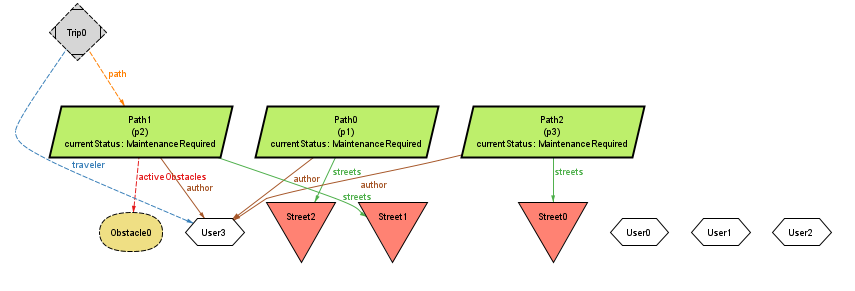
\includegraphics[width=1.1\linewidth]{RASD/Images/Alloy/Timeframe0.png}
    \label{fig:placeholder}
\end{figure}
\noindent
User3 takes a trip on Path1 but decides to discard it; therefore, no report is submitted. The status of all paths remains unchanged, and the set of obstacles remains the same.

\newpage
\textbf{Timeframe 1 (focus on tie and add/remove obstacles):}
\begin{figure}[!h]
    \centering
    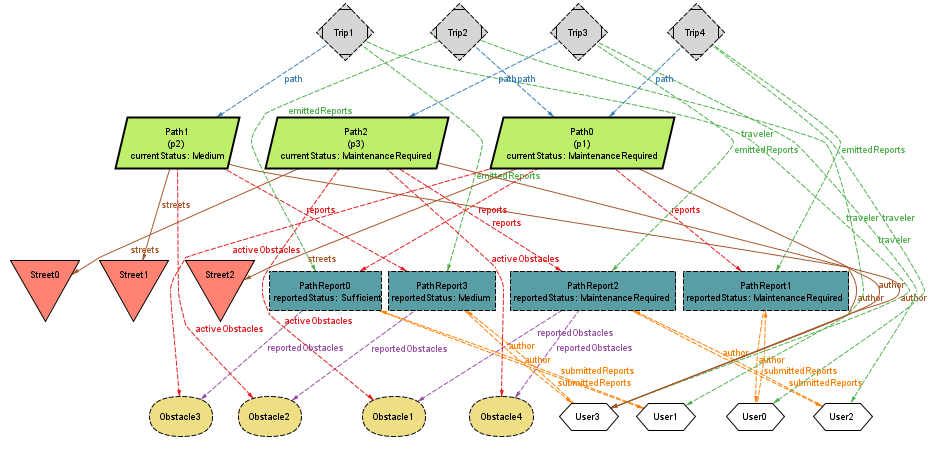
\includegraphics[width=1.1\linewidth]{RASD/Images/Alloy/Timeframe1.png}
    \label{fig:placeholder}
\end{figure}

\noindent
User0 emits a report on Path0 with status = 'Manteinance Required'. \\
User1 emits a report on Path0 with status = 'Sufficient' and one obstacle (Obstacle3).\\
User2 emits a report on Path2 with status = 'Manteinance Required' and two obstacles (Obstacle1 and Obstacle4).\\
User3 emits a report on Path1 with status = 'Medium' and one obstacle (Obstacle 2), and it removes Obstacle0.\\
As a result, Path1 and Path2 take the status of the single report associated, while since there is a tie in the count of report statuses for Path0, it is assigned the lower of the two statuses (Maintenance Required).\\
In addition, Obstacle0 will be replaced with Obstacle3 in Path1, Obstacle1 and Obstacle4 have been added to Path2, and Obstacle2 has been added to Path1.

\newpage
\textbf{Timeframe 2 (focus on merging):}
\begin{figure}[!h]
    \centering
    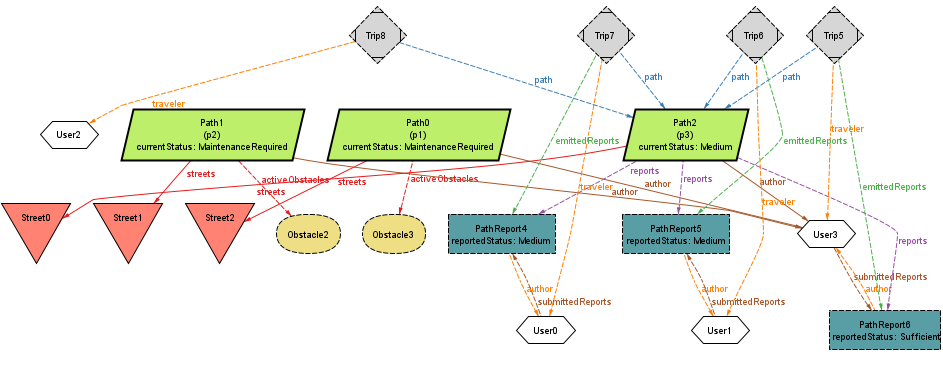
\includegraphics[width=1.1\linewidth]{RASD/Images/Alloy/Timeframe2.png}
    \label{fig:placeholder}
\end{figure}
\\
User0 emits a report on Path2 with status = 'Medium'. \\
User1 emits a report on Path0 with status = 'Medium'.\\
User3 emits a report on Path2 with status = 'Sufficient'.\\
User2 makes a trip on Path2 but decides to discard it, therefore no report is submitted.\\
As a result, the status of Path2 is updated to Medium according to the majority vote, while the remaining paths are unaffected.